\chapter{Snow Surface Dielectric Constant Estimation From Full Polarimetric SAR Data}
\section{Introduction}
The dielectric constant of snow is a function of frequency, temperature, water content (volumetric), density, ice-particles and water inclusions shape~\cite{Hallikainen86}. Several studies have been conducted to measure the microwave dielectric properties of snow and ice since 1950's~\cite{Cumming52,sweeny1974measurements,tobarias1978determination,linlor1980permittivity}. The propagation of Electromagnetic (EM) waves in snow is governed by its dielectric constant $\varepsilon = \varepsilon{'}-j\varepsilon{''}$. Snow is a heterogeneous mixture of air, ice and liquid water. Dry snow consists of ice particles and air, whereas wet snow contains liquid water as a third component. Microwaves strongly respond to this change due to the liquid water content in snow~\cite{Hallikainen86,tiuri1984complex,Hallikainen87}. The dielectric behavior of water and ice is described by a Debye type relaxation spectrum~\cite{stiles1980dielectric}. Passive and active microwave remote sensing systems have been widely used to determine the extent, water equivalent, and wetness of snow cover. Passive analysis of snowpack were made in the frequency range of 5 to 94 GHz~\cite{ulaby1980active,stiles1980active,tiuri1982theoretical}, whereas, active measurements were conducted for frequencies between 1 to 36 GHz~\cite{ulaby1980active,matzler1982towards} for both dry and wet snow conditions. 

The snow surface dielectric constant is an important parameter for avalanche studies, hydrological modeling and flood monitoring. Remote sensing using polarimetric SAR data has great potential in determining the extent and the properties of snow. The radar backscatter coefficient has been shown to be very useful for quantitative estimation of snowpack parameters~\cite{Stiles1980,ulaby1986microwave}. Radar backscattering effects on geographical areas, relief, aspect angle, layover and shadow has also been studied~\cite{Koskinen97,Nagler2000,small2011flattening}. The snow volume scattering has been modeled by a discrete particle model which was experimentally justified at C-band~\cite{Kendra98,Koskinen2000}. Snow wetness and snow water equivalent have been inferred from C-band polarimetric SAR data~\cite{Shi95,Shi2000}. Very recently a new snow wetness estimation model has been proposed which utilize the polarimetric SAR decomposition technique~\cite{surendar2015wetness}. 

In this paper we propose a new method to estimate snow surface dielectric constant from polarimetric SAR data. The novelty of the method is realized by the introduction of the effective degree of polarization estimated by unitary rotation of the coherency matrix. This technique leads to maximize the number of surface scattering pixels for inversion.  A ratio of the Bragg's coefficients $B_{HH}$ and $B_{VV}$ as a function of the local incidence angle $\theta_{i}$ and dielectric constant $\varepsilon_{r}$ is related to the dominant scattering type magnitude $\alpha_{s1}$~\cite{TOUZI2007}. An inversion technique is then used to estimate the dielectric constant $\varepsilon_{r}$. A similar approach~\cite{Hajnsek2003} has been proposed to invert soil surface parameters from polarimetric SAR data using the Cloude-Pottier entropy ($H$) and alpha ($\alpha$). 

\section{Methodology}
\subsection{Dominant Scattering Mechanism}
In this study dominant scattering type amplitude is considered to characterize scattering from snow. In order to understand this it is very essential to know that which layers of snow/ice are primarily responsible for this scattering. The scattering from volume is mainly observed from dry snow in which microwave can penetrate 10 m at 10 GHz~\cite{rott1987possibilities}. However, small variations in liquid water content in snow significantly reduces the penetration depth. A depth of an order of one wavelength for liquid water content of 2-4$\%$ by volume has been reported in~\cite{rott1987possibilities}. A penetration depth of 13.8~cm for 1$\%$ and 4.9~cm for 3$\%$ liquid water by volume for ERS-1 C-band SAR data have been reported in~\cite{rott1995monitoring}.

The dominant scattering type amplitude ($\alpha_{s1}$) is obtained from the eigenvalue/eigenvector based incoherent target decomposition (ICTD) theorem proposed in~\cite{TOUZI2007}. In general, ICTD is used to express the averaged scattering mechanism given by a $3\times3$ coherency matrix $\langle[{\mathbf{T}}]\rangle$ as a sum of independent scattering components~\cite{Cloude92NATO,Cloude96,TOUZI2007}. The $\alpha$--$\beta$ scattering model proposed in~\cite{Cloude96} differs from the scattering model proposed in~\cite{TOUZI2007} for non-symmetric targets. The scattering type parameter $\alpha$ introduced by Cloude-Pottier is infact a function of the symmetric scattering type magnitude $\alpha_{s}$ and the helicity $\tau_{m}$. However, the dominant scattering type $\alpha_{s1}$ obtained from the first eigenvector (corresponding to $p_{1}$ with $p_{3}<p_{2}<p_{1}$, where $p_{i}=\lambda_{i}/\sum_{1}^{3}\lambda_{i}$) is similar to $\alpha_{1}$ for $\tau_{m}\simeq0$. In this study, while considering the dominant scattering type from snow surface, a subset $\alpha_{s1}^{B}$~\eqref{eq:alpha_subset} of $\alpha_{s1}$ has been considered which characterizes Bragg's scattering. 
\begin{equation}
\alpha_{s1}^{B}=\Big\{\{\alpha_{s1} \in [0,90^\circ]: p_{1}\ge 0.7\} \le 20^\circ\Big\}
\label{eq:alpha_subset}
\end{equation}
Therefore, $\alpha_{s1} \in \alpha_{s1}^{B}$ has been considered for analysis in this study. The $\alpha_{s1}$ image for the study site is shown in Fig.~\ref{Fig:alpha_s1}. It can be clearly that seen that $\alpha_{s1} \le 20^\circ$ for most of the areas. Moreover, it can be seen that in the higher altitudes ($> 4000$~m.a.s.l) $\alpha_{s1} \ge 40^\circ$ which may be due to volume scattering from dry snowpack. In the next section the effective (optimum) degree of polarization is estimated by unitary transformation of the coherency matrix. 

%===============================================%
\subsection{Optimum Degree of Polarization}
The degree of polarization ($m$) is defined as the ratio of the (average) intensity of the polarized portion of the wave to that of the (average) total intensity of the wave. For a completely polarized EM wave, $m = 1$ and for a completely unpolarized EM wave, $m = 0$. In between these two extreme cases, the EM wave is said to be partially polarized, $0 \le m \le 1$. Very recently it has been shown in~\cite{Bhattacharya15} that the degree of polarization can be suitably used as a criteria for the adaptive nature of a model based decomposition. 

In some model-based decompositions~\cite{Arii11,An10,YAMAGUCHI2011,Lee2011,singh13,Chen14,Bhattacharya15_SD_Y4O}, the $3\times3$ multi-look coherency $\mathbf{\langle[T]\rangle}$ or the covariance $\mathbf{\langle[C]\rangle}$ matrices (where $\langle\dots\rangle$ denotes ensemble averaging) is rotated by a real matrix $[{\mathbf{R}}(\theta)]$~\eqref{eq:R_theta} about the radar line of sight (LOS). The angle $\theta$ is obtained by minimizing the $T_{33}(\theta)$ component of $\mathbf{\langle[T]\rangle}$. 
\begin{equation}
[{\mathbf{R}}(\theta)] = \left[ \begin{array}{ccc}
1 &0 & 0 \\
0 & \cos(2\theta) & \sin(2\theta) \\
0 & -\sin(2\theta) & \cos(2\theta)
\end{array}\right] 
\label{eq:R_theta} 
\end{equation}
The fundamental idea behind such compensation is to minimize the cross-polarization component. The orientation compensation can be used to reduce the overestimation of the volume power in a model-based decomposition to a certain extent and increase the double-bounce power. 
In the proposed method~\cite{Bhattacharya15}, after the real rotation, two complex unitary transformation matrices $[{\mathbf{R}}(\phi_1)]$ and $[{\mathbf{R}}(\phi_2)]$~\eqref{eq:R_phi_2} were applied to the $\langle[{\mathbf{T}}(\theta)]\rangle$ matrix,
\begin{align*}
\langle[{\mathbf{T}}(\phi_1)]\rangle&=[{\mathbf{R}}(\phi_1)]\langle[{\mathbf{T}}(\theta)]\rangle[{\mathbf{R}}(\phi_1)]^{-1} \quad \mbox{and},\\[0.4em] 
\langle[{\mathbf{T}}(\phi_2)]\rangle&=[{\mathbf{R}}(\phi_2)]\langle[{\mathbf{T}}(\theta)]\rangle[{\mathbf{R}}(\phi_2)]^{-1}
\end{align*}
where the angles $\phi_{1}$ and $\phi_{2}$ are obtained similarly by minimizing the  $T_{33}(\phi_{1})$ and the $T_{33}(\phi_{2})$ components respectively. 
\begin{gather}
[{\mathbf{R}}(\phi_1)] = \left[ \begin{array}{ccc}
1 & 0 & 0 \\
0 & \cos(2\phi_1) & j\sin(2\phi_1) \\
0 & j\sin(2\phi_1) & \cos(2\phi_1)
\end{array}\right] \label{eq:R_phi_1} \\[0.5em] 
[{\mathbf{R}}(\phi_2)] = \left[ \begin{array}{ccc}
\cos(2\phi_2) & 0 & j\sin(2\phi_2) \\
0 & 1 & 0 \\
j\sin(2\phi_2) & 0 & \cos(2\phi_2)
\end{array}\right] 
\label{eq:R_phi_2}
\end{gather}

In order to compute the degree of polarization, the coherency matrices $\langle[{\mathbf{T}}(\phi_1)]\rangle$ and $\langle[{\mathbf{T}}(\phi_2)]\rangle$ are transformed into a $4\times4$ Mueller matrices $\langle[{\mathbf{M}}(\phi_1)]\rangle$ and $\langle[{\mathbf{M}}(\phi_2)]\rangle$ respectively. 

The received Stokes vectors $\mathbf{G_{H}^{r}}=\begin{bmatrix} g_{H1}^{r} & g_{H2}^{r} & g_{H3}^{r} & g_{H4}^{r}
\end{bmatrix}^{T}$ and $\mathbf{G_{V}^{r}}=\begin{bmatrix}
g_{V1}^{r} & g_{V2}^{r} & g_{V3}^{r} & g_{V4}^{r}
\end{bmatrix}^T$ for a horizontal and a vertical  polarizations respectively are related to the
transmit Stokes vectors $\mathbf{G_{H}^{t}} = \begin{bmatrix}
1 & 1 & 0 & 0
\end{bmatrix}^T$ and $\mathbf{G_{V}^{t}} = \begin{bmatrix}
1 & {-1} & 0 & 0
\end{bmatrix}^T$ for linear horizontal and vertical polarizations respectively by $\mathbf{G_{H/V}^{r}}=\mathbf{\langle[M]\rangle}\mathbf{G_{H/V}^{t}}$. The degree of polarization of a received EM wave for a horizontally (H) and a vertically (V) transmitted wave is defined as $m_{H}$ and $m_{V}$~\eqref{eq:dop} respectively and $m_{E}$ is the effective degree of polarization~\eqref{eq:dop_h_v}.
\begin{gather}
m_{H} = \frac{\Big(\sum_{i=2}^{4}({g_{Hi}^{r}})^2 \Big)^{1/2}}{g_{H1}^{r}},\quad\label{eq:dop}
m_{V} = \frac{\Big(\sum_{i=2}^{4}({g_{Vi}^{r}})^2 \Big)^{1/2}}{g_{V1}^{r}}\\[0.1em] 
m_{E} = \Bigg(\frac{m_{H}^{2}+m_{V}^{2}}{2}\Bigg)^{1/2}
\label{eq:dop_h_v}
\end{gather}

The two independent $m_{E}$'s which are obtained from the Mueller matrices, $\langle[{\mathbf{M}}(\phi_1)]\rangle$ and $\langle[{\mathbf{M}}(\phi_2)]\rangle$ are compared and the maximum among the two $m_{E}^{opt}$ is retained for that particular pixel as shown in Fig~\ref{Fig:DOP}. Along with $\alpha_{s1} \in \alpha_{s1}^{B}$, the $m_{E}^{opt}$ is used to delineate the pixels which are then used to estimate the dielectric constant by an inversion technique shown in the next section.

The two independent $m_{E}$'s which are obtained from the Mueller matrices, $\langle[{\mathbf{M}}(\phi_1)]\rangle$ and $\langle[{\mathbf{M}}(\phi_2)]\rangle$ are compared and the maximum among the two $m_{E}^{opt}$ is retained for that particular pixel as shown in Fig~\ref{Fig:DOP}. Along with $\alpha_{s1} \in \alpha_{s1}^{B}$, the $m_{E}^{opt}$ is used to delineate the pixels which are then used to estimate the dielectric constant by an inversion technique shown in the next section.
\begin{figure*}[!h]
	\centering
	\subfloat[$\alpha_{s1}$\label{Fig:alpha_s1}]{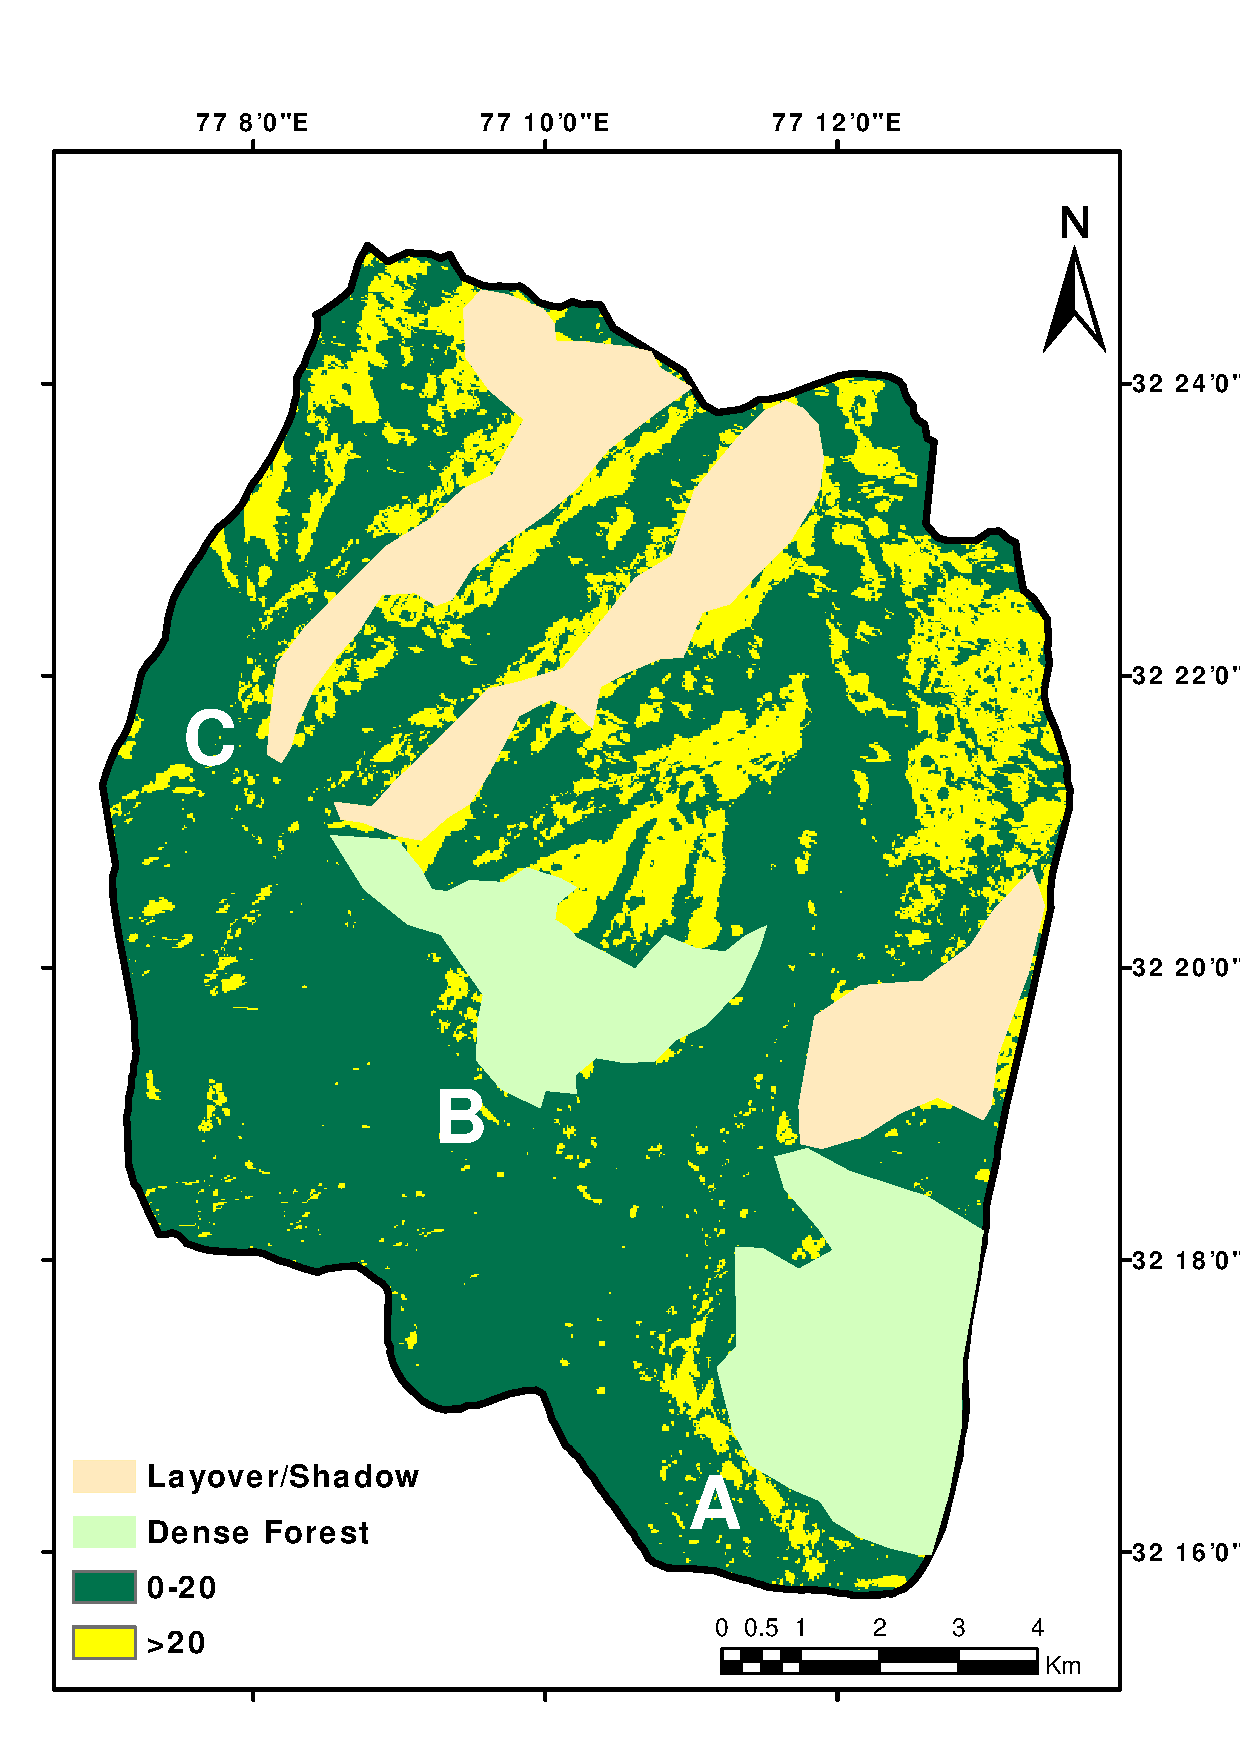
\includegraphics[width=0.49\columnwidth]{Figures_SSD/alpha_8feb13}} \hspace{1mm}
	\subfloat[$m_{E}^{opt}$\label{Fig:DOP}]{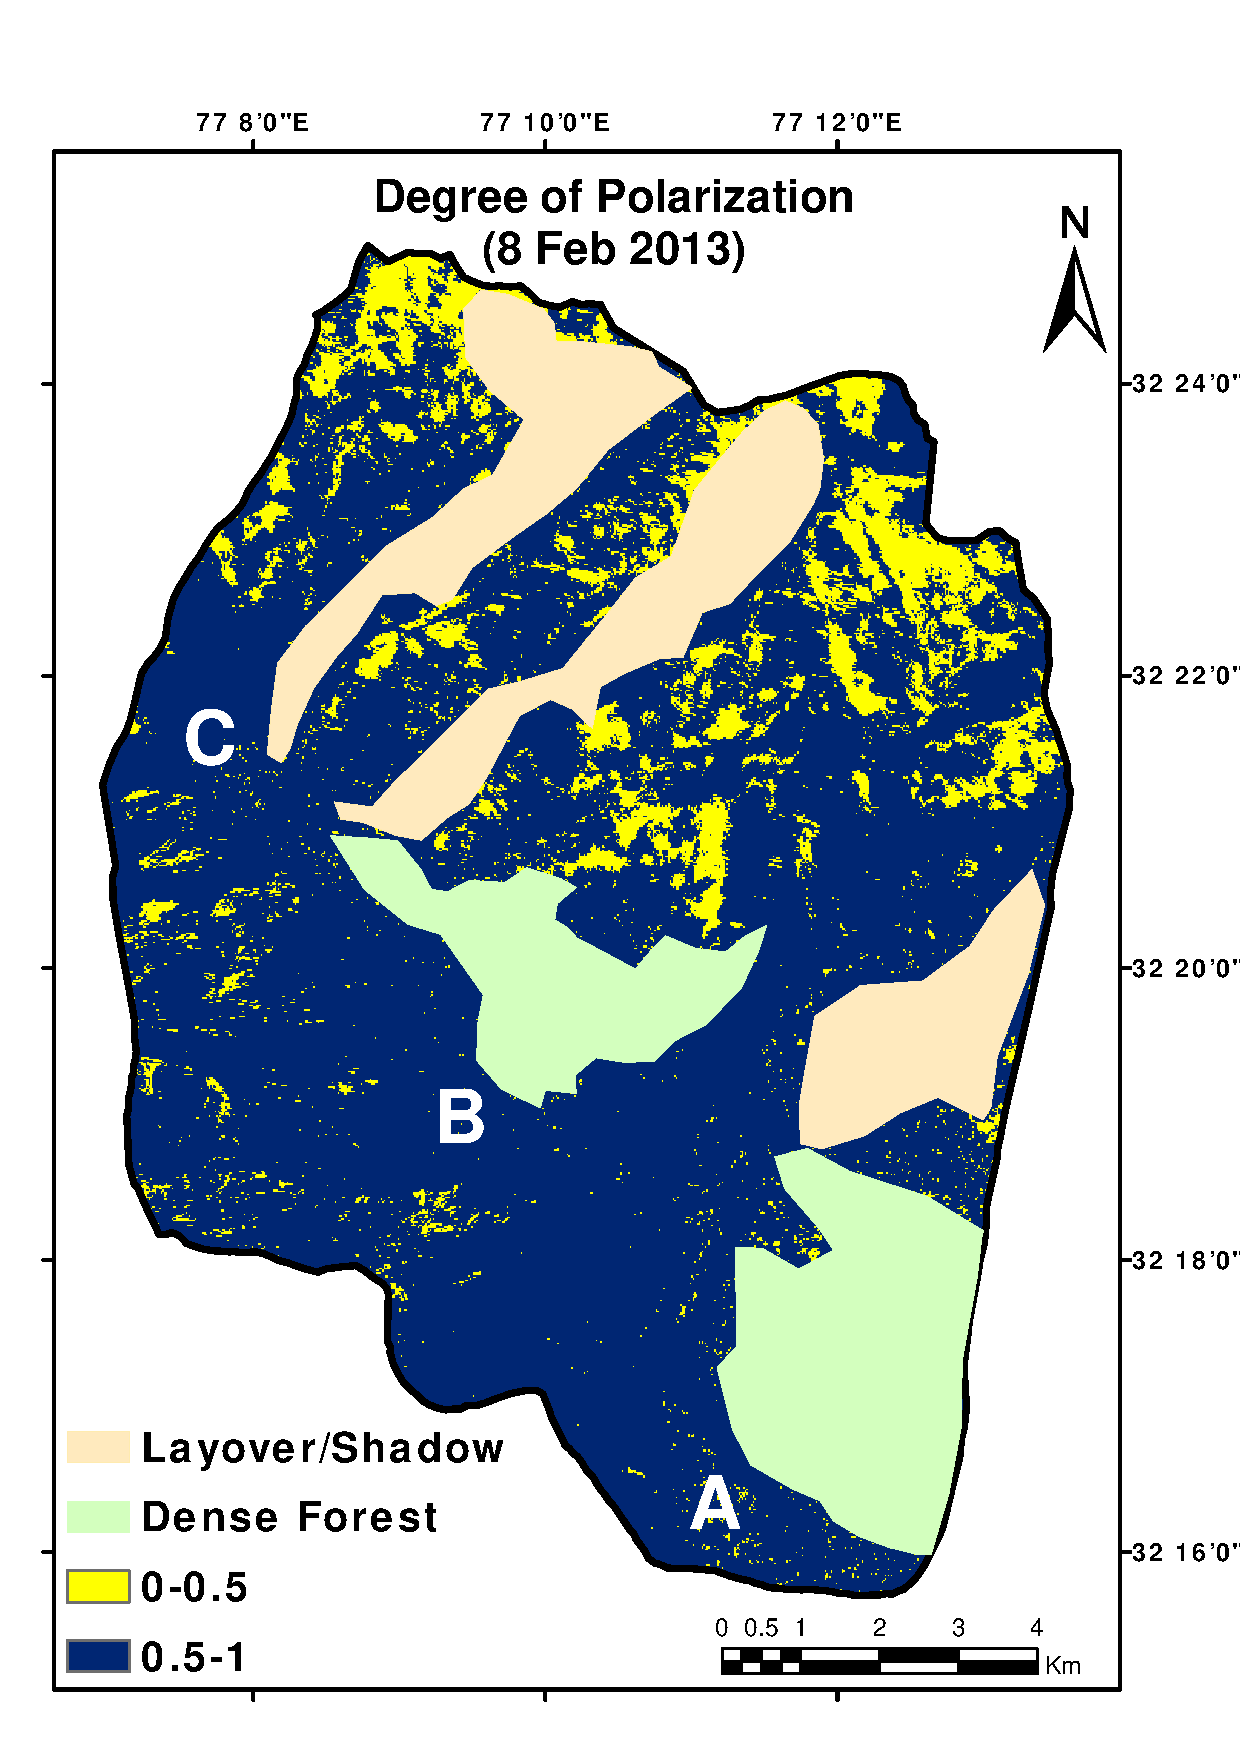
\includegraphics[width=0.49\columnwidth]{Figures_SSD/DOP_8feb2013}} 
	\hspace{1mm}
	\subfloat[$\alpha_{s1} \mbox{vs.} m_{E}^{opt}$\label{Fig:dop_alpha}]{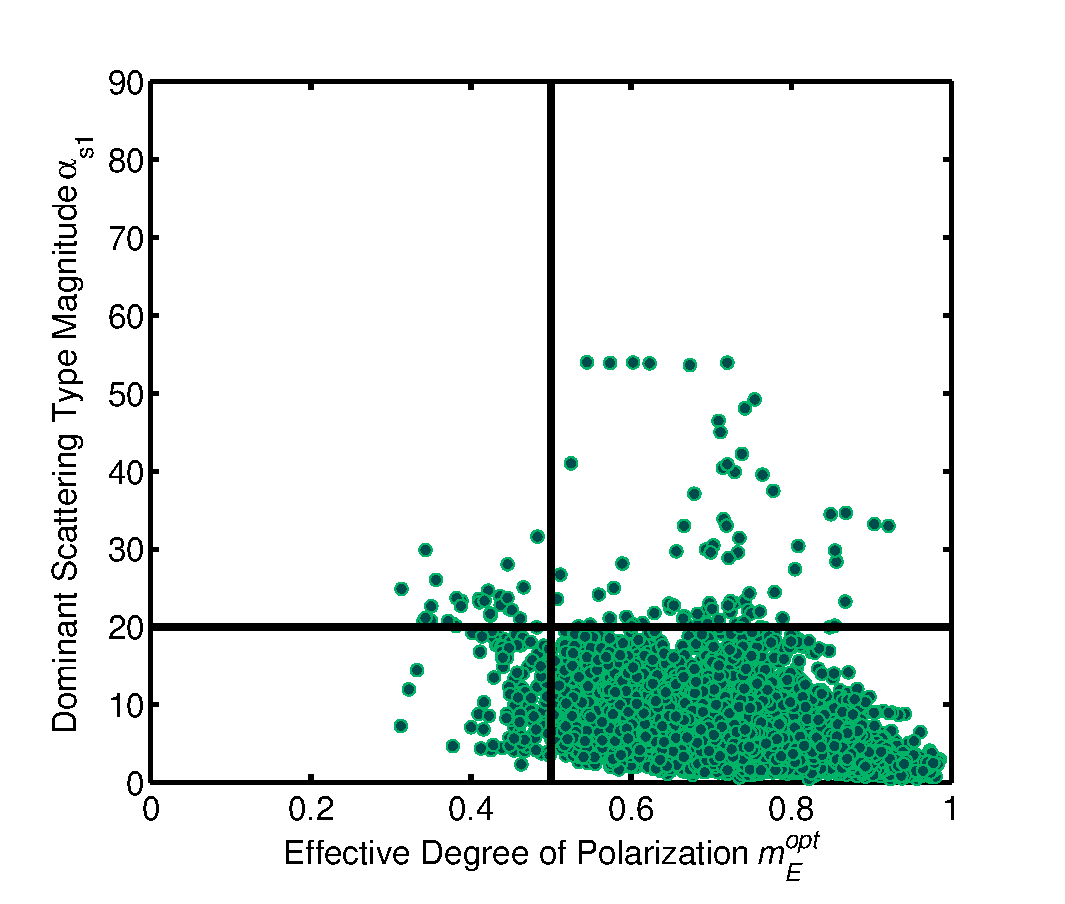
\includegraphics[width=0.65\columnwidth]{Figures_SSD/dop_alpha}} 
	\caption{(a). The dominant scattering type magnitude, (b) the optimum degree of polarization and (c) the $\alpha_{s1} \mbox{vs.} m_{E}^{opt}$ plot. The points A, B and C on the maps are the three observatory locations over the study area.}
	\label{fig:results_1}
\end{figure*}	
%===============================================%
\subsection{Snow Surface Dielectric Constant}
The small perturbation or Bragg rough surface scattering~\cite{tsang1985theory} is defined for large (compared to the incident wavelength $\lambda$) surface facets where the rms surface roughness $s$ is small compared to $\lambda$. This is usually expressed in terms of the wavenumber $k$ and for all practical applications $ks < 0.3$. The backscattered power depends only on a certain frequency component which pertains to the surface roughness spectrum (the Fourier transform of the surface profile). Moreover, the surface roughness is implicit in the Fourier transform of the surface profile and it is similar to both the polarization channels (HH and VV). Hence, a simple ratio of the co-polarized channels (eg. HH/VV) will be only a function of the local incidence angle $\theta_{i}$ and the snow surface dielectric constant $\varepsilon_{r}$~\cite{cloude2009polarisation}. This can also be expressed by relating the roll-invariant dominant scattering type amplitude $\alpha_{s1}$ to the Bragg's coefficients $B_{HH}$ and $B_{VV}$ as shown in~\eqref{eq:alphas1_bragg} and~\eqref{eq:bragg_coefficients_1}--~\eqref{eq:bragg_coefficients_2} respectively.
\begin{equation}
\alpha_{s1}=\tan^{-1}\Bigg(\Bigg|\frac{B_{HH}-B_{VV}}{B_{HH}+B_{VV}}\Bigg|\Bigg), \quad \alpha_{s1} \in \alpha_{s1}^{B}
\label{eq:alphas1_bragg}
\end{equation}
\begin{subequations}
	\begin{align}
	B_{HH} =& \frac{\mbox{cos}\theta_{i} - \sqrt{\varepsilon_{r} - \mbox{sin}^2\theta_{i}}}{\mbox{cos}\theta_{i} + \sqrt{\varepsilon_{r} - \mbox{sin}^2\theta_{i}}} \label{eq:bragg_coefficients_1}\\
	B_{VV} =& (\varepsilon_{r}-1)\frac{\mbox{sin}^2\theta_{i} - \varepsilon_{r}(1 + \mbox{sin}^2\theta_{i})}{\left[\varepsilon_{r}\mbox{cos}\theta_{i} + \sqrt{\varepsilon_{r} - \mbox{sin}^2\theta_{i}}\right]^2} \label{eq:bragg_coefficients_2}
	\end{align}
\end{subequations}
Following this, the snow surface dielectric constant $\varepsilon_{r}$ is numerically obtained by inverting~\eqref{eq:alphas1_bragg} for only those pixels which lie in the region of $\alpha_{s1}^{B}$ and $m_{E}^{opt} > 0.5$. This can be clearly seen in Fig.~\ref{Fig:dop_alpha} for samples from the study area used in this paper for the 8 Feb data . 

This methodology can be justified by the fact that approximately $9-10\%$ increase in the number of pixels have been obtained compared to the original data $(\langle[{\mathbf{T}}]\rangle)$ for all the data sets used in this study by using the criteria of optimum degree of polarization $m_{E}^{opt}$. These pixels lies in the region of $\alpha_{s1}^{B}$ and have been correctly inverted to obtain $\varepsilon_{r}$. 

%\section{Results and discussion}
%Fine resolution full-polarimetric Radarsat-2 C-band SAR data acquired on 7 Feb. 2012, 8 Feb. 2013 and 18 Feb. 2014 over the Manali-Dhundi area in Himachal Pradesh India are used in this study. The 3$\times$3 coherency matrix was generated from the single-look complex data. A multi-looking factor of 3 in the range and 4 in the azimuth directions were used to make a square pixel and the Lee-Refined filter is applied to remove the speckle noise. The local incidence angle map is generated while performing the Range Doppler terrain correction using the 30~m SRTM DEM and the Layover/Shadow areas were masked. The range and azimuthal pixel spacing were approximately 20~m (19.7~m$\times$20.9~m) respectively after processing. Field campaigns were conducted to collect near-real time in-situ measurements using the snowfork instrument and a hand held GPS with the all three Radarsat-2 data acquisitions for consecutive three winter seasons from 2012 to 2014. 
%
%\begin{figure*}[!h]
%	\centering
%	\subfloat[\label{Fig:Snow_surf_diel_7Feb2012}]{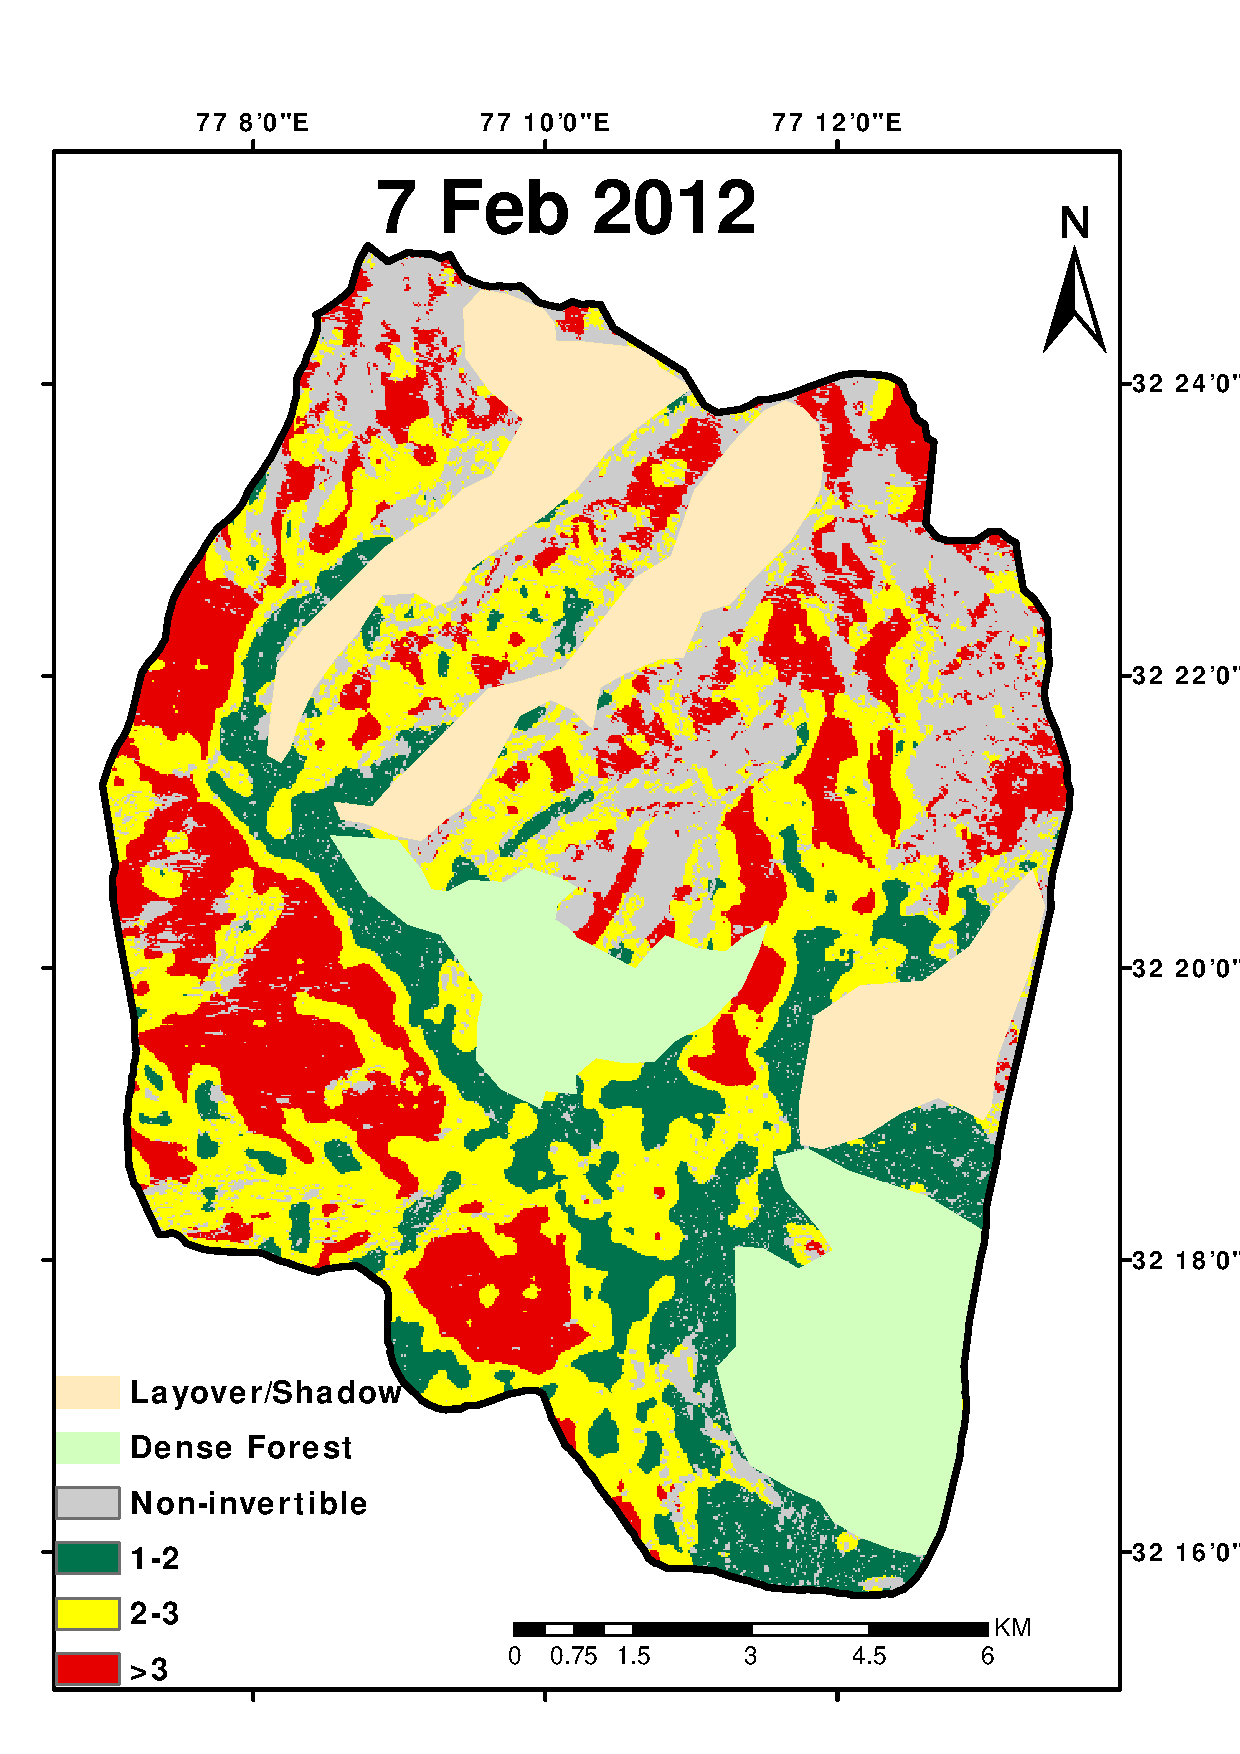
\includegraphics[width=0.49\columnwidth]{Figures_SSD/7Feb2012}} \hspace{1mm}
%	\subfloat[\label{Fig:Snow_surf_diel_8Feb2013}]{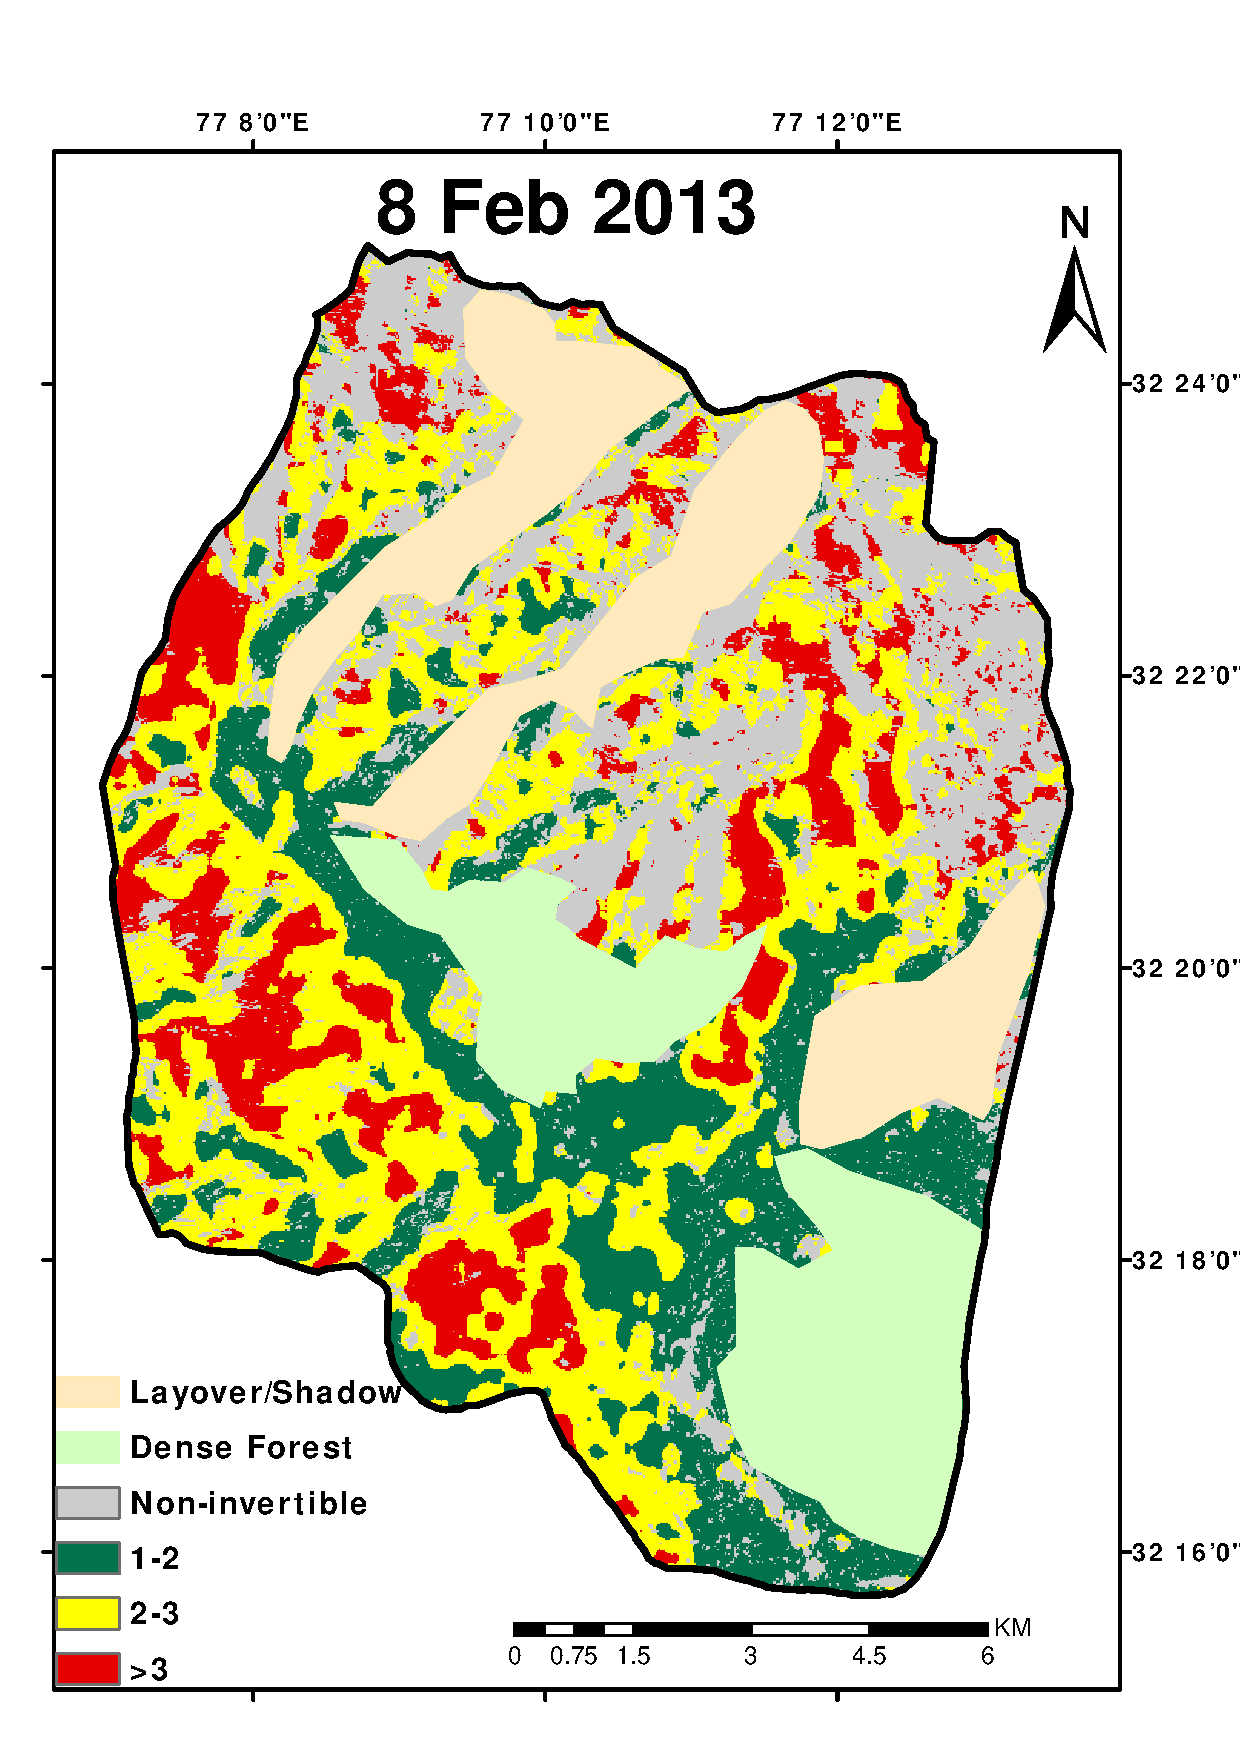
\includegraphics[width=0.49\columnwidth]{Figures_SSD/8feb2013}} \hspace{1mm}
%	\subfloat[\label{Fig:Snow_surf_diel_18Feb2014}]{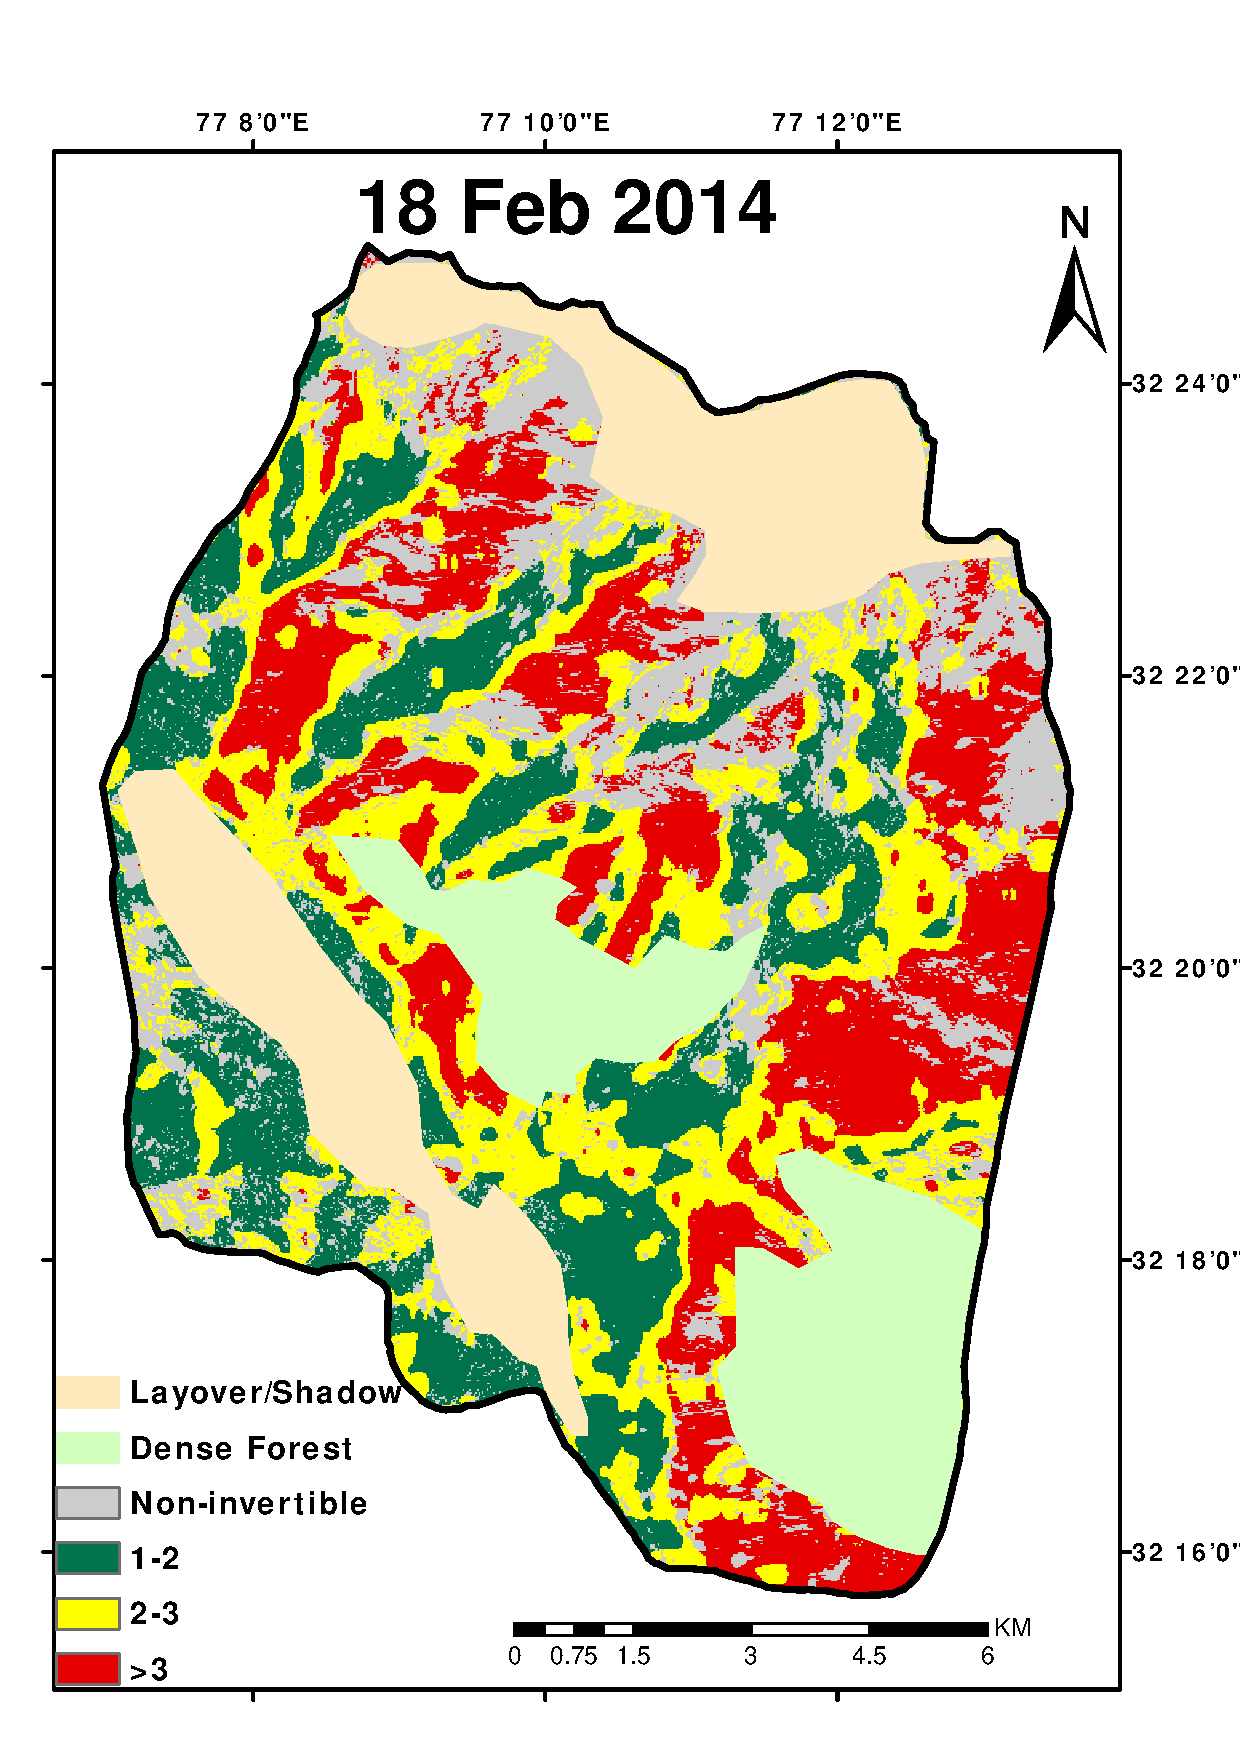
\includegraphics[width=0.49\columnwidth]{Figures_SSD/18feb2014}} 
%	\caption{Temporal snow surface dielectric constant maps estimated over the Manali-Dhundi area for three consecutive winters.}
%	\label{fig:results_2}
%\end{figure*}	
%
%The estimated snow surface dielectric constant maps for 7 Feb. 2012, 8 Feb. 2013 and 18 Feb. 2014 using the proposed algorithm are shown in Fig.~\ref{Fig:Snow_surf_diel_7Feb2012}, ~\ref{Fig:Snow_surf_diel_8Feb2013} and ~\ref{Fig:Snow_surf_diel_18Feb2014} respectively. The notations A, B and C on the maps indicate the observatory locations at Bahang, Solang and Dhundi which are at an altitude of 2006~m, 2446~m and 2896~m respectively. The percentage of areas covered with different snow surface dielectric constant ranges for all the three data sets are presented in Table~\ref{table:snow_dielectric_rang}. It is observed that in all the maps, the snow cover with the surface dielectric constant range of 2--3 are in most of the areas. Generally in the month of February, the snowfall with considerable temperature variation is observed over the Indian Himalayan region. This condition will initiate the melt-freeze process in the snowpack. So, the surface snow dielectric constant values are mostly in the range of 1.5--3 in the month of February over the study region. 
%
%On 7 Feb. 2012 the descending pass data was acquired around 6.18 AM IST (Indian Standard Time) along with the in-situ measurements collected around the Bahang observatory. The estimated surface dielectric constant values over the Bahang observatory are in the range of 1.5--2 which are closer to the measured values. It can be observed that around 18$\%$ of the area shows the surface dielectric constant values of $>$3. These are mostly over high altitudes along with high slopes (Fig.~\ref{Fig:DEM} and Fig.~\ref{Fig:Slop}). The Dhundi observatory shows more than 20~cm melting on 6 Feb. 2012. This melting rate might be higher over the slopes than the flat observatory areas. However, during the descending pass acquisition, the observed low temperature ($<-2^\circ$C) might have frozen the melted water over the snow surface within few centimeters. This frozen depth should be lower over the slopes compared to the flat areas. The observed high dielectric constant over the slopes is due to the presence of wet snow layers on the top of the snowpack. These conditions clearly distinguishes between the lower surface dielectric constant over the flat areas and high over the slopes. High wetness and density values over the same slopes have been reported in~\cite{surendar2015wetness,surendar2015density} for the same dataset.
%
%The dielectric constant map for 8 Feb. 2013 (Fig.~\ref{Fig:Snow_surf_diel_8Feb2013}) almost follows the same trend as compared to the previous year (7 Feb. 2012). The observed maximum temperature on 7 Feb. 2013 at Bahang, Solang and Dhundi were 11$^\circ$C, 7$^\circ$C and 6$^\circ$C with a melting of around 11~cm, 23~cm and 9~cm respectively. However, the observed low temperature during the descending pass acquisition at the Bahang ($-3^\circ$C), Solang ($-7.5^\circ$C) and Dhundi ($-7^\circ$C) have frozen the snowpack surface similar to the previous year. The snow surface dielectric constant map for the ascending pass data acquired on 18 Feb. 2014 at 6.30 PM IST is shown in Fig.~\ref{Fig:Snow_surf_diel_18Feb2014}. The different range of dielectric constant values with snow covered areas for 18 Feb 2014 is shown in Table~\ref{table:snow_dielectric_rang}. It can be seen from the map (Fig.~\ref{Fig:Snow_surf_diel_18Feb2014}) that mostly the areas with high slopes on the eastern side shows high dielectric constant range ($>$3). This is because of the direct sun's illumination on the eastern slopes during sunset just before the acquisition. 
%
%A total of 20 in situ measurements were collected in near real time with the satellite data for the three consecutive years to validate the proposed snow surface dielectric constant estimation algorithm. 
%The snow surface dielectric constant estimated by the proposed algorithm along with in situ measurements is plotted in Fig.~\ref{Fig:Validation_plot}. The dielectric constant of top 5~cm of the snowpack is considered as the snow surface dielectric constant for validation of the proposed method. The correlation coefficient between the measured and the estimated snow surface dielectric constant is 0.95 at 95$\%$ confidence interval with a root mean square error (RMSE) of 0.20. 
%
%Temporal variation of the snow surface dielectric constant map for a 2015 winter season is shown in Figure.\ref{Fig:29Jan2015}, \ref{Fig:22Feb2015} and \ref{Fig:18Mar2015}. It can be observed that the variation of surface dielectric constant values mainly over the high altitude regions which may be because of the fresh snowfall in January and continues melting in march. 
%
%\begin{table}[!th]
%	\caption{Percentage of area with the snow surface dielectric constant range}
%	\begin{center}
%		\begin{tabular}{|c|c|c|c|} \hline
%			Dielectric Range & \multicolumn{3}{c|}{Area ($\%$)} \\
%			\cline{2-4}
%			& 7 Feb. 2012 & 8 Feb. 2013 & 18 Feb. 2014 \\ \hline
%			1-2 &	13.77 &	17.03 &	17.54 \\ \hline
%			2-3 &	24.44 &	25.26 &	19.93 \\ \hline
%			$>$3&   18.31 &	11.91 &	17.53 \\ \hline
%			Dense forest cover & 12.59 &	12.59 &	12.59 \\ \hline
%			Layover/Shadow & 12.67 &	12.67 &	15.42 \\ \hline
%		\end{tabular}
%	\end{center}
%	\label{table:snow_dielectric_range}
%\end{table}
%\begin{figure*}[!h]
%	\centering
%	\subfloat[\label{Fig:DEM}]{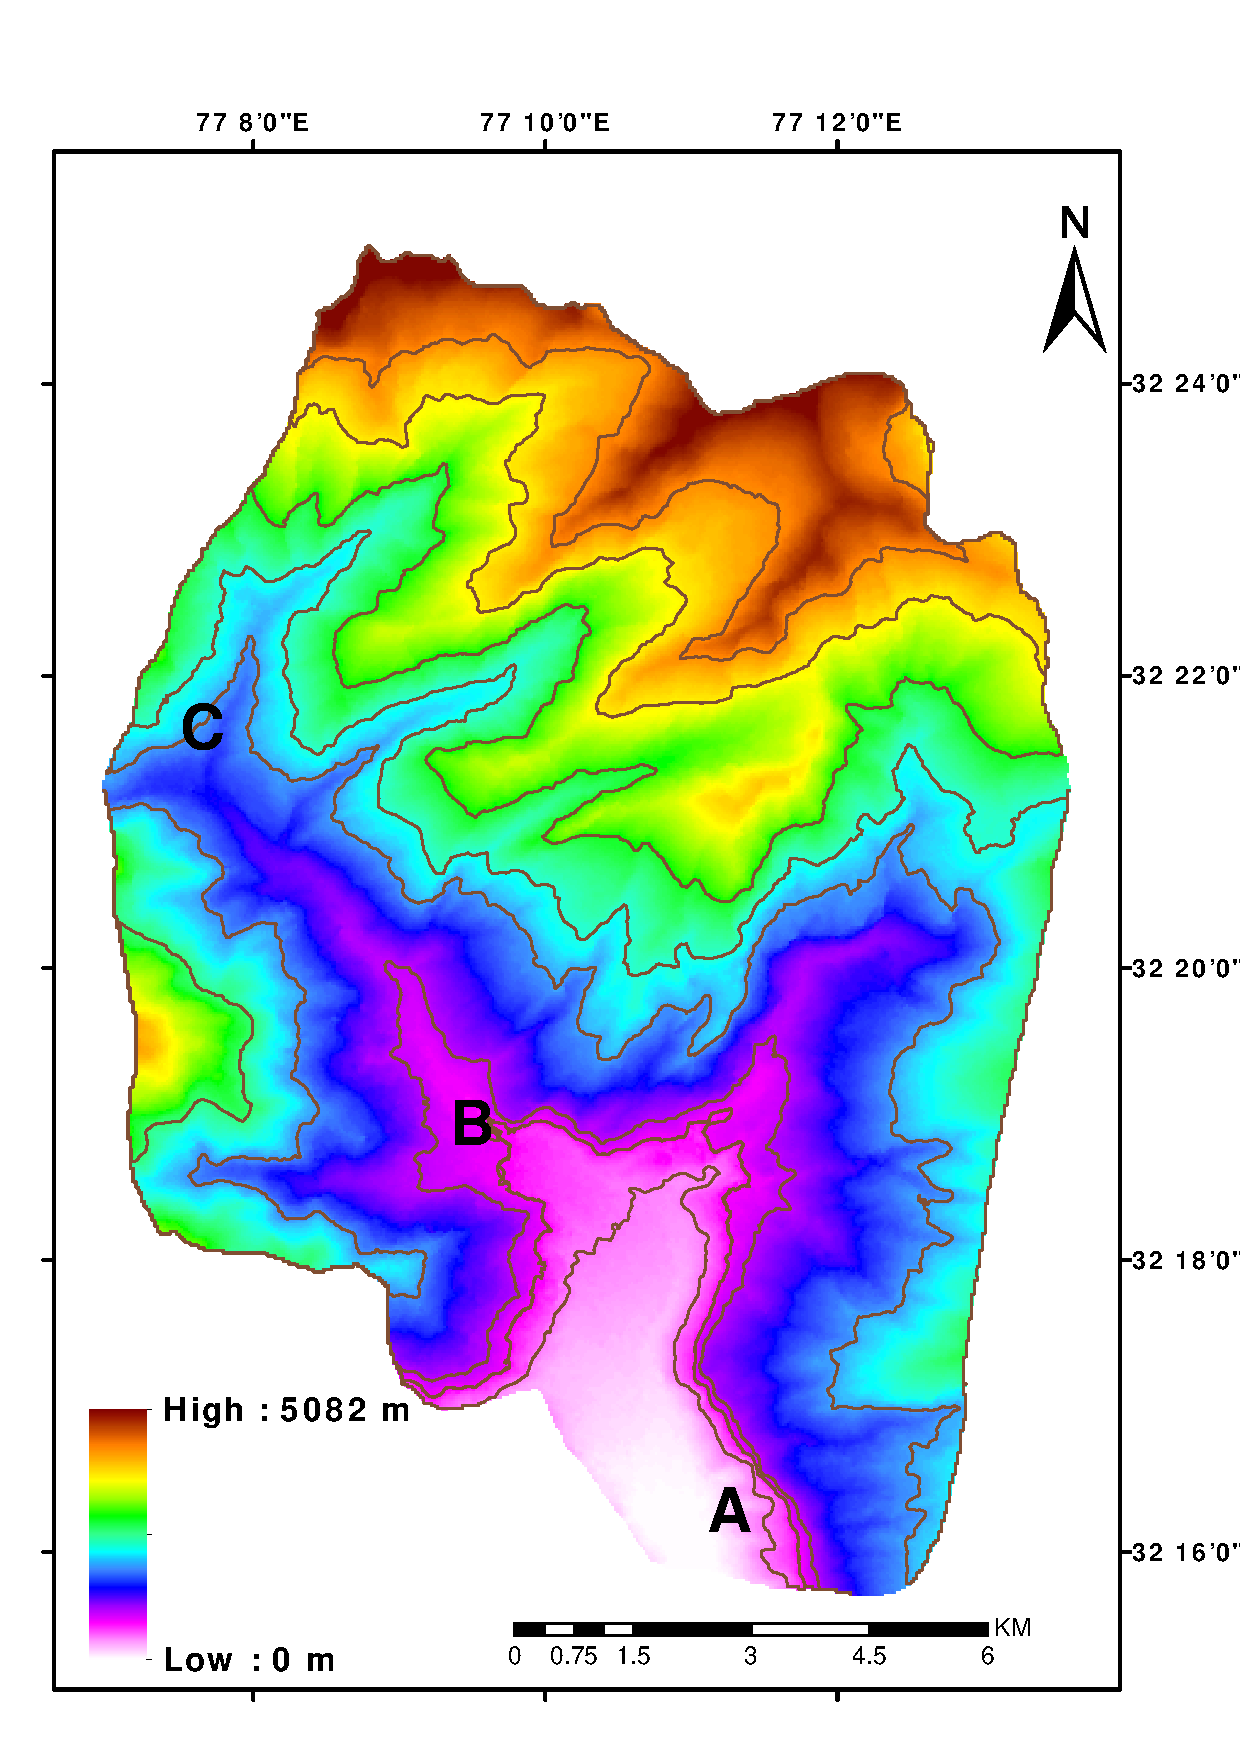
\includegraphics[width=0.49\columnwidth]{Figures_SSD/DEM_subset}} \hspace{1mm}
%	\subfloat[\label{Fig:Slop}]{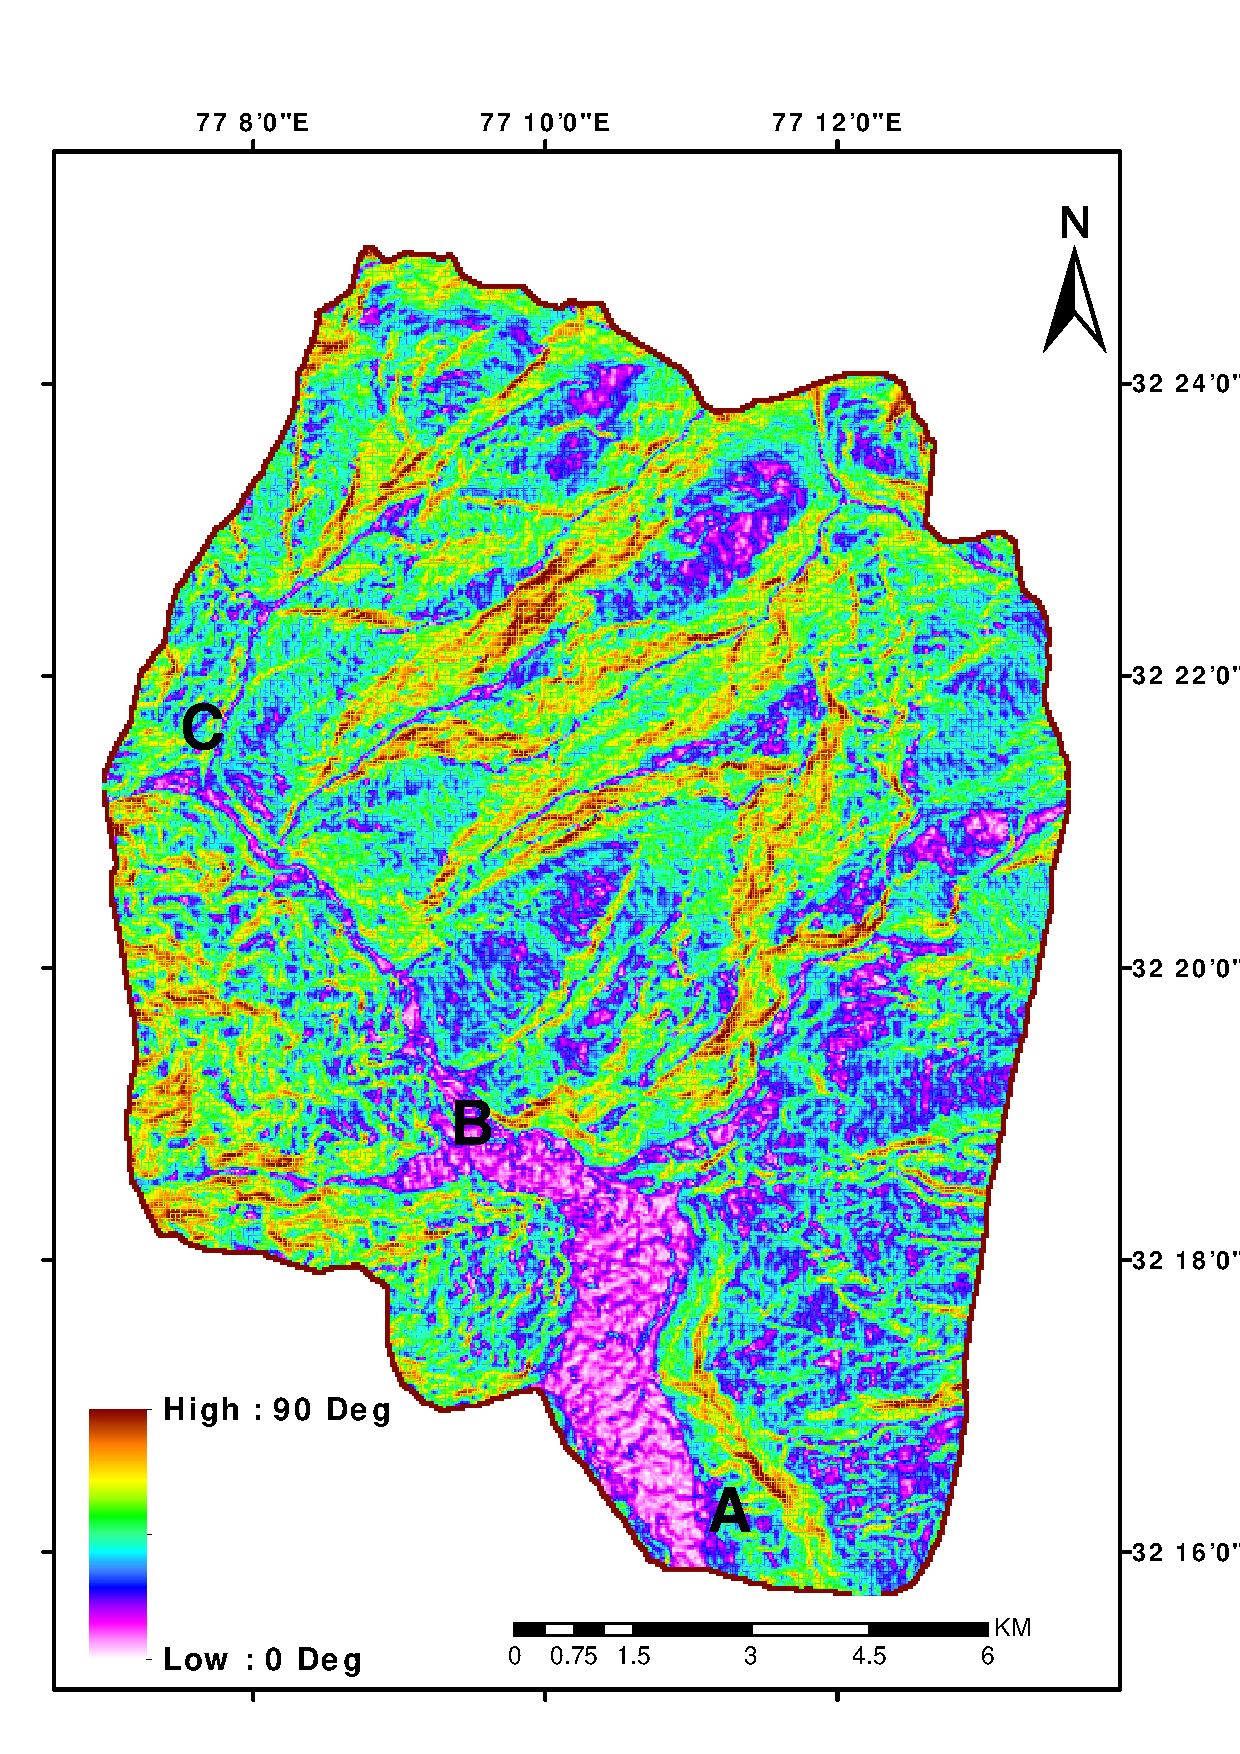
\includegraphics[width=0.49\columnwidth]{Figures_SSD/Slop}} \hspace{1mm}
%	\subfloat[\label{Fig:Validation_plot}]{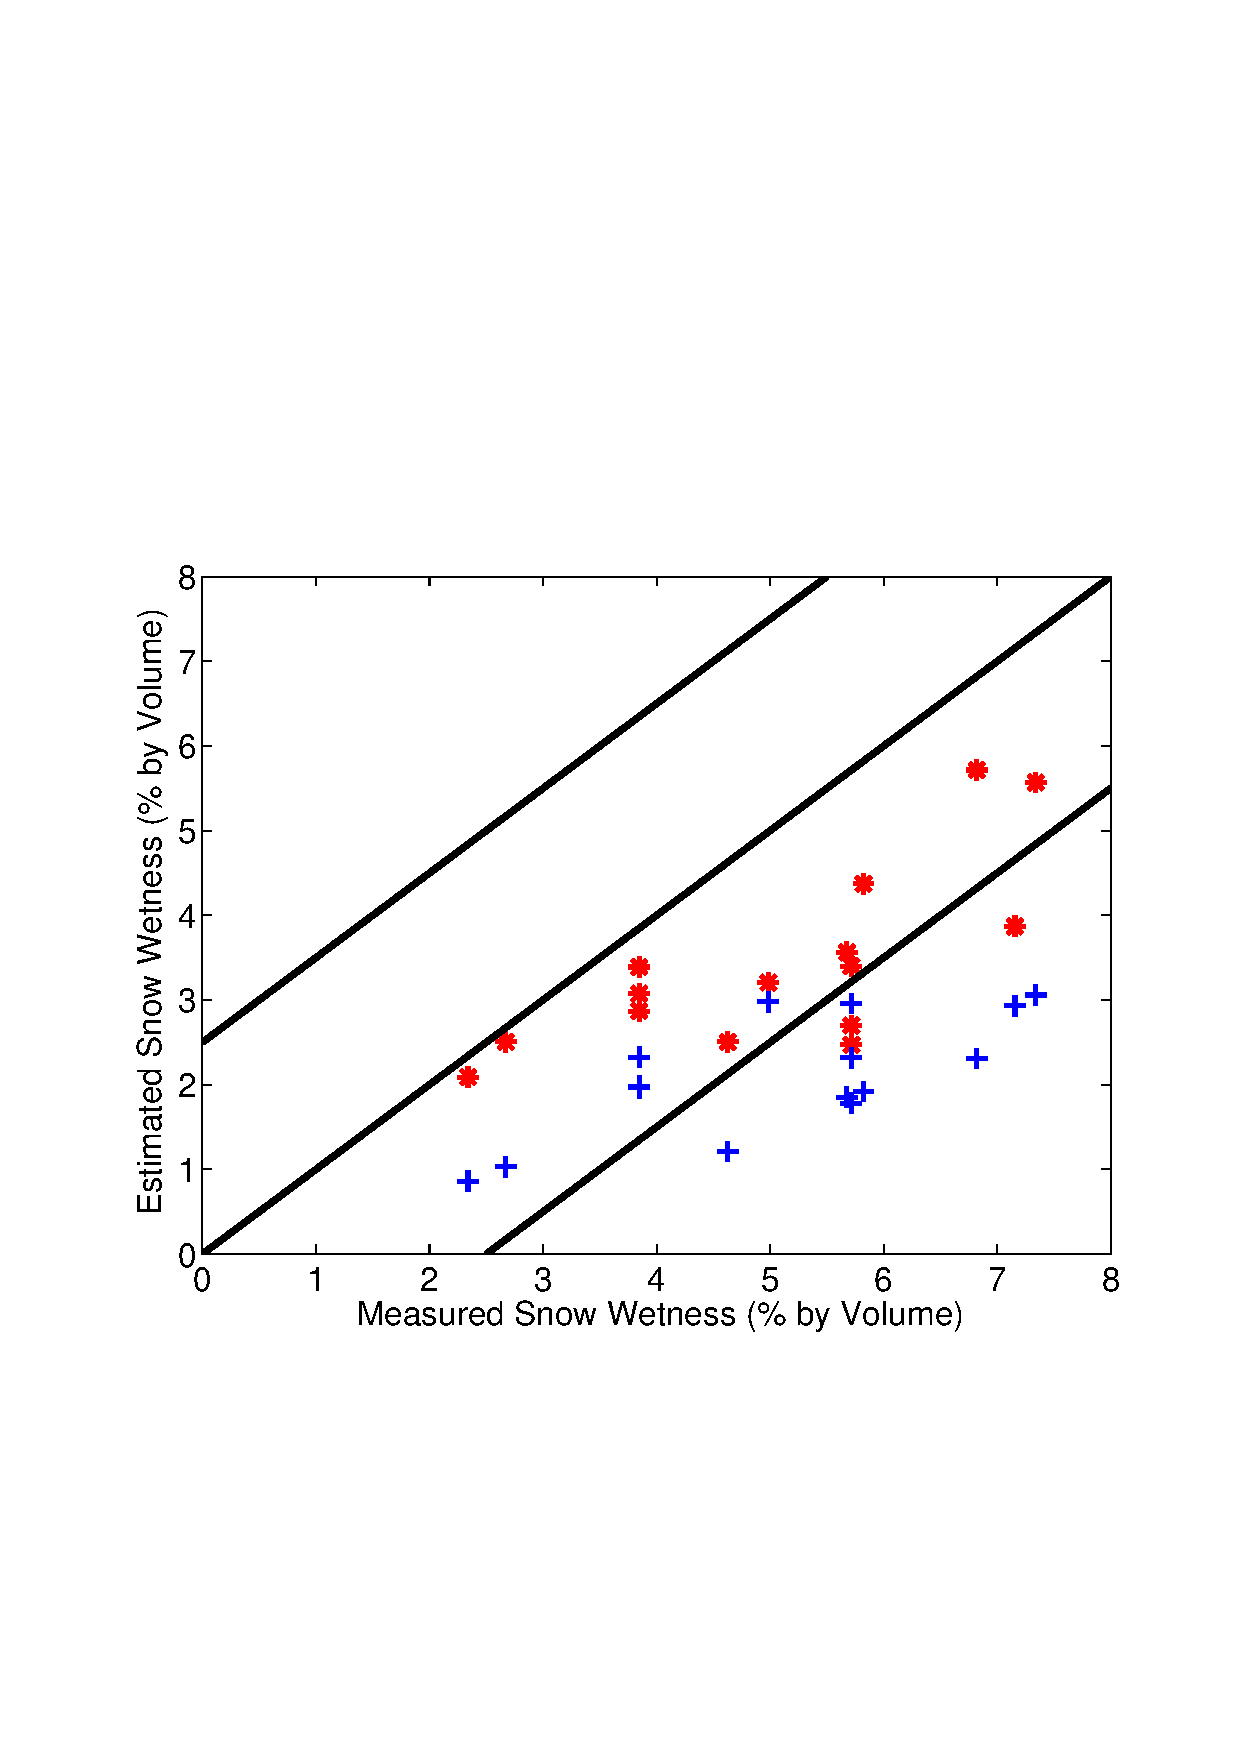
\includegraphics[width=0.65\columnwidth]{Figures_SSD/validation_plot.png}}
%	\caption{(a). 30 m SRTM DEM and (b) slope map over the study area. (c) Validation Plot }
%	\label{fig:results_3}
%\end{figure*}
%
%\begin{figure*}[!h]
%	\centering
%	\subfloat[\label{Fig:29Jan2015}]{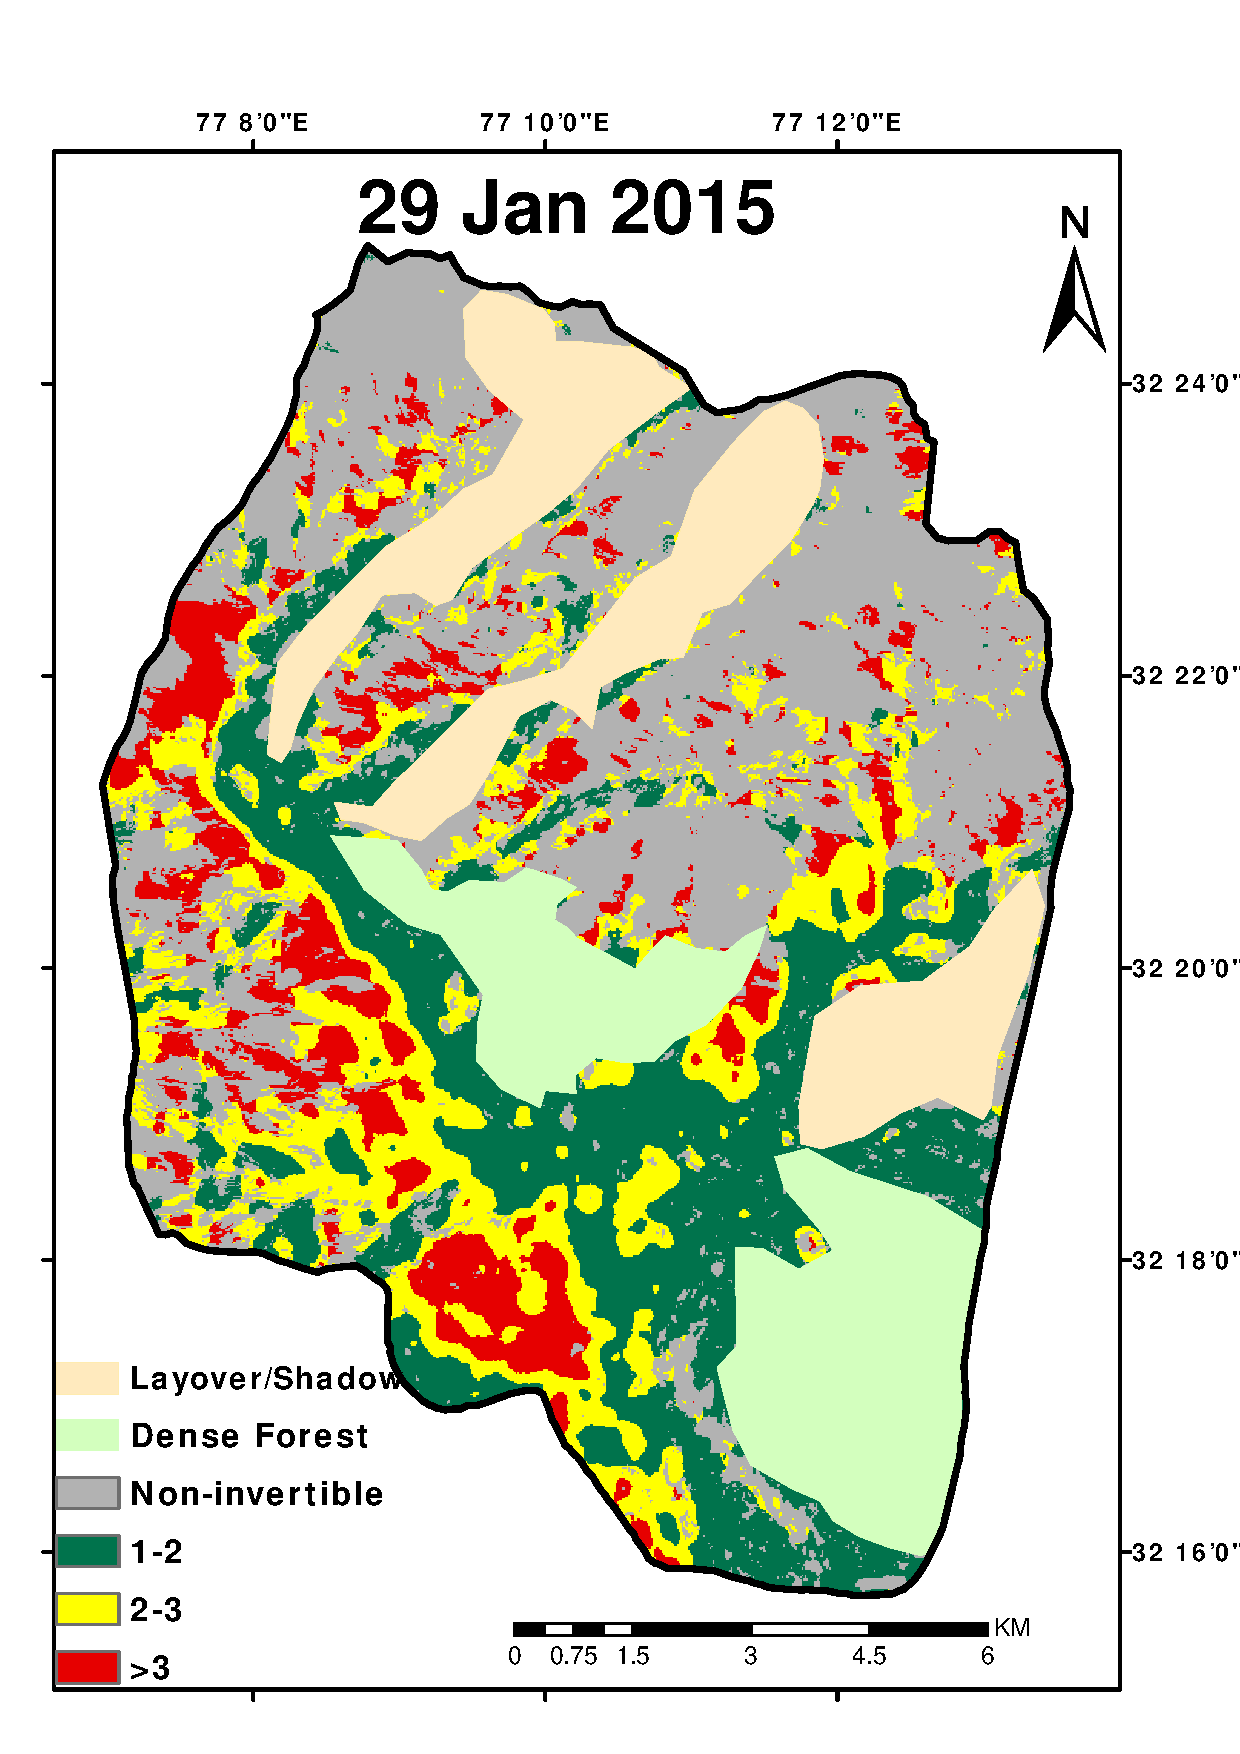
\includegraphics[width=0.49\columnwidth]{Figures_SSD/SSD_29Jan15}} \hspace{1mm}
%	\subfloat[\label{Fig:22Feb2015}]{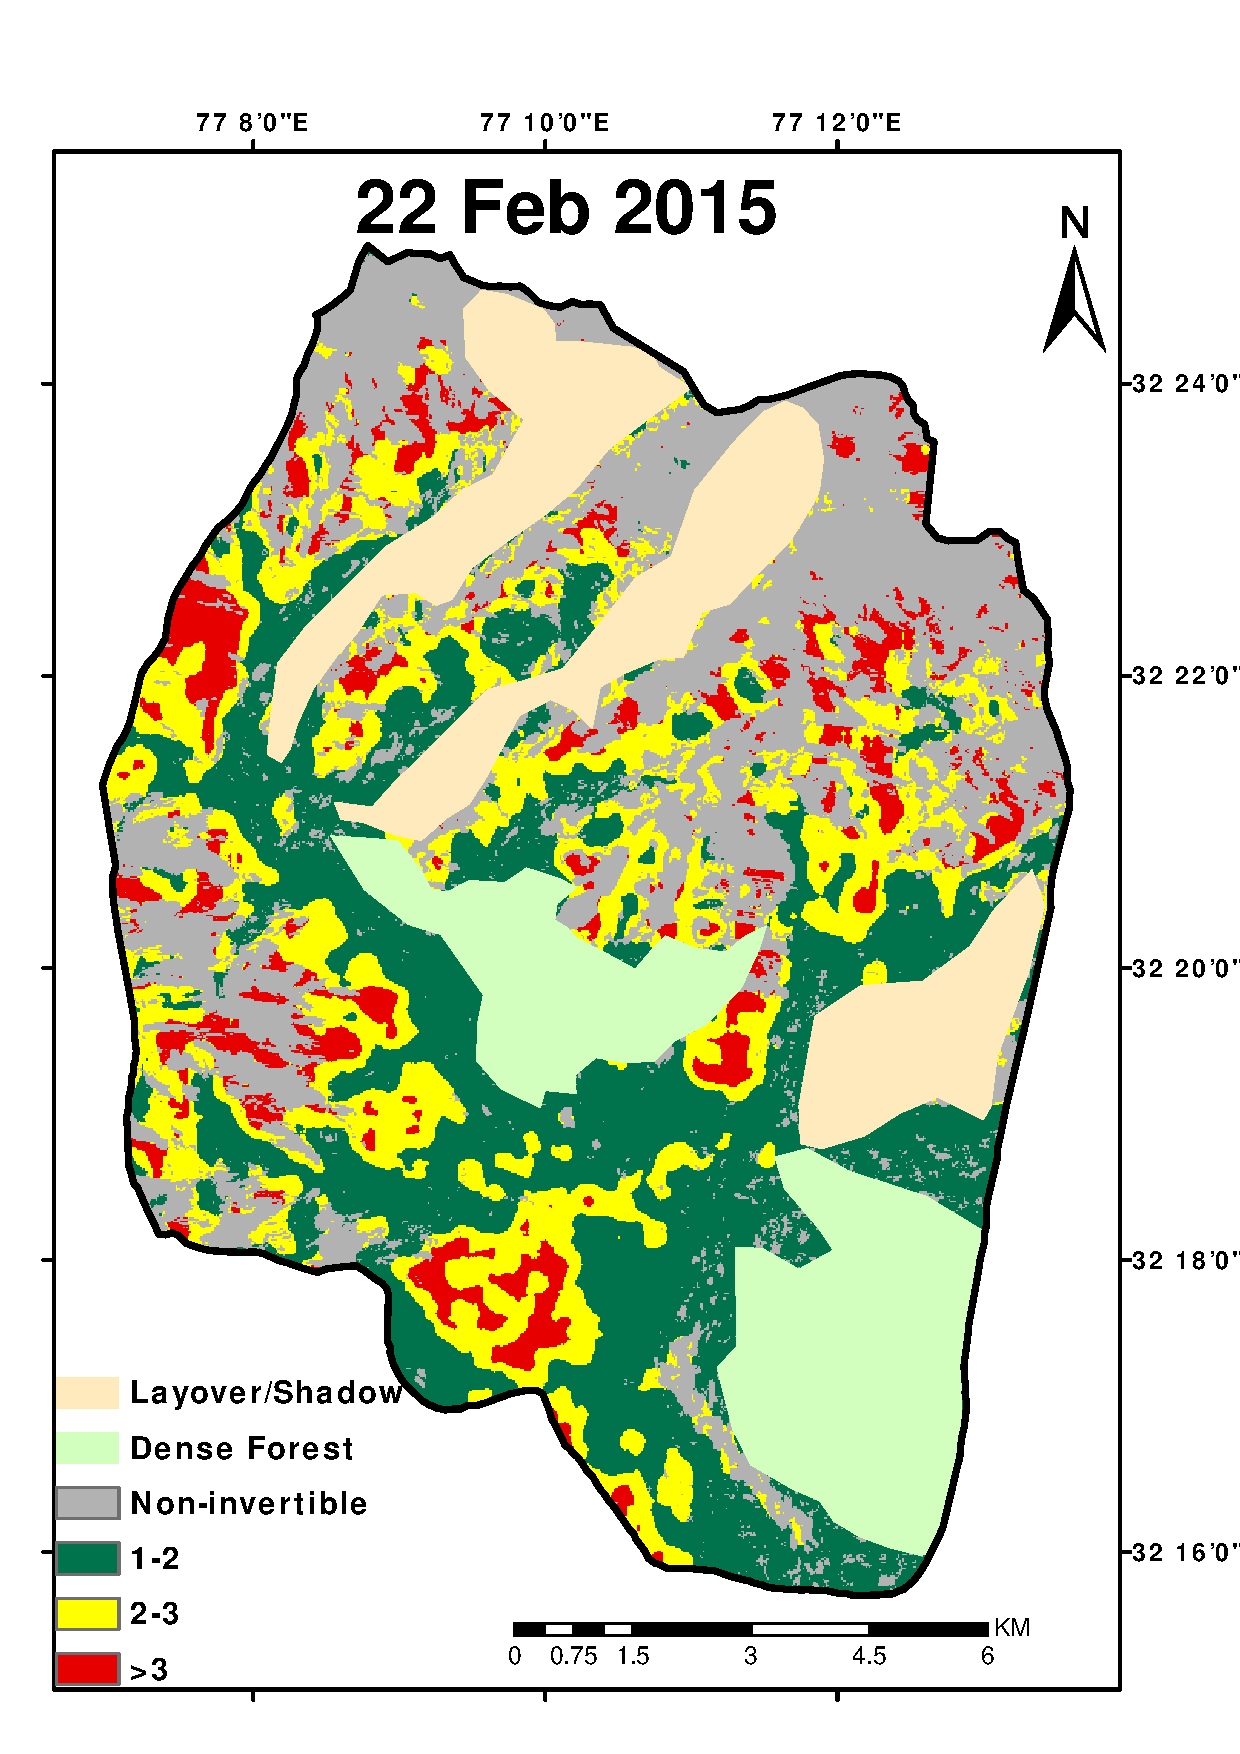
\includegraphics[width=0.49\columnwidth]{Figures_SSD/SSD_22Feb15}} 
%	\hspace{1mm}
%	\subfloat[\label{Fig:18Mar2015}]{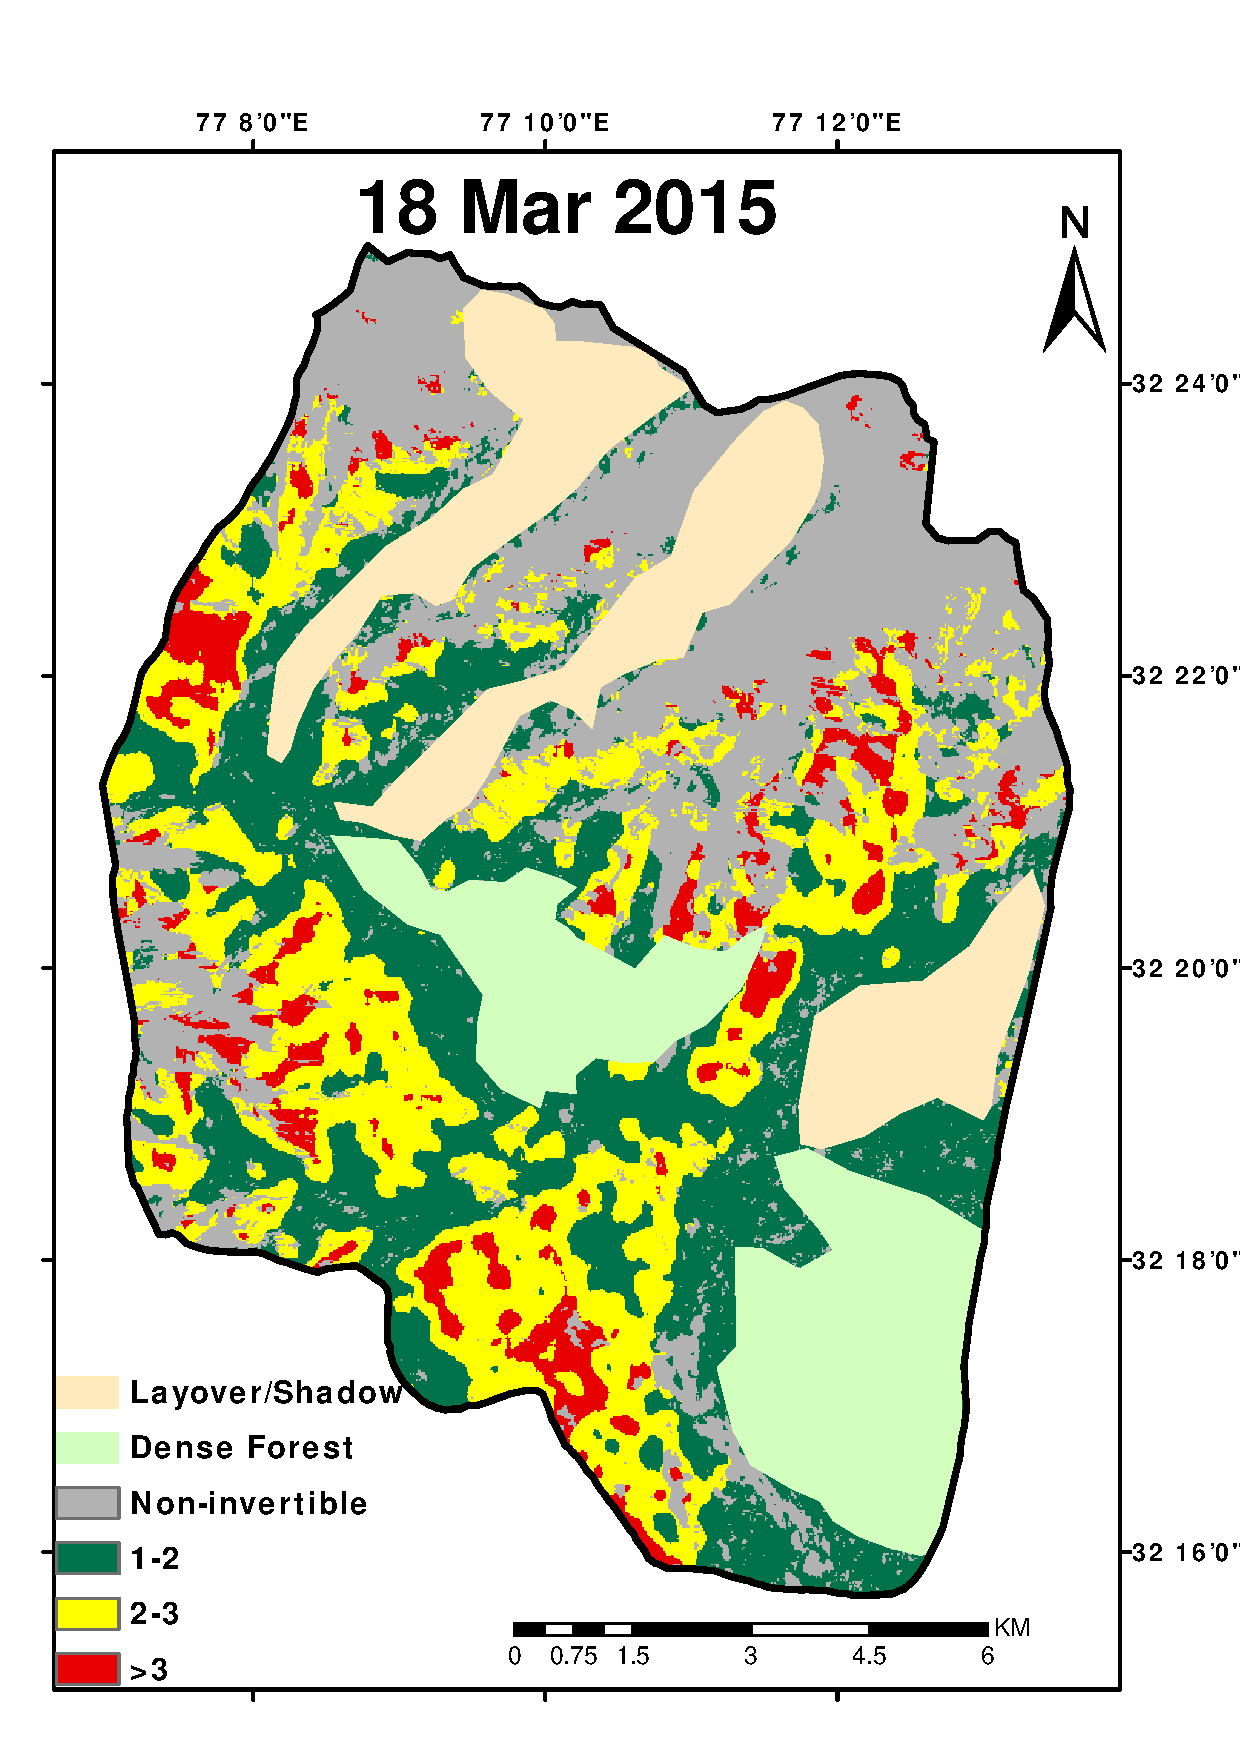
\includegraphics[width=0.49\columnwidth]{Figures_SSD/SSD_18Mar15}} 
%	\caption{Multi-temporal snow surface dielectric constant maps in a season over the study area}
%	\label{fig:Multi_temporal_SSD}
%\end{figure*}
%\section{Conclusion}
%In this chapter, a new methodology for snow surface dielectric constant estimation from  full-polarimetric C-band SAR data is proposed. The dominant scattering type amplitude ($\alpha_{s1}$) is used to characterize dominant snow scattering mechanism and the optimum degree of polarization ($m_{E}^{opt}$) has been used as a criteria for the selection of maximum surface scattering pixels which were used for the inversion of the snow surface dielectric constant. The optimized degree of polarization have increased the number of pixels for inversion by approximately 9--10$\%$ compared to the original data. The proposed algorithm was applied to three consecutive winter acquisitions of full-polarimetric fine resolution Radarsat-2 data over Indian Himalayan region. The correlation coefficient between the measured and the estimated snow surface dielectric constant was found to be 0.95 at 95$\%$ confidence interval with a root mean square error (RMSE) of 0.20. 